   
  \chapter{Teorie a technologie}
  V této části si přiblížíme technologie potřebné k návrhu a vývoji webové služby specifikované v zadání práce. Postupně budou vysvětleny všechny zásadní pojmy, které pomůžou čtenáři doplnit znalosti v dané problematice.
  
  \section{REST}
	Representational state transfer (dále jen REST) je architektura pro komunikaci  mezi distribuovanými systémy. Termín zavedl R. T. Fielding ve své disertační práci\cite{restThesis}, kde toto rozhraní bylo taktéž popsáno a vymezeno. Mimo jiné stanovil i těchto 5 základních pravidel, která by měla být dodržena, aby se aplikace nazývala RESTful\cite{rest}:
	\begin{itemize}
		\item Klient-Server (Client-Server) - Toto omezení staví na principu oddělení zodpovědností (Separation of Concerns), nebo-li je klientská část starající se o uživatelské rozhraní je oddělena od serverové části přistupující k databázi. Zlepšuje škálovatelnost sytému a zjednodušuje použitelnost na různých platformách.
		\item Bezestavovost (Stateless) - Každý požadavek musí přenášet všechna související data, server totiž neuchovává žádné informace o nynějším spojením a každý požadavek bere jako nový.
		\item Keš (Cache) - Data přenášená v odpovědi mohou být označená jako kešovatelná, tudíž si je klient může uložit a kdykoliv použít znova.
		\item Jednotné rozhraní (Unified interface) - Základem tohoto omezení je princip HATEOAS (Hypermedia As The Engine Of Application State), který říká, že klient nepotřebuje znát pravidla komunikace dopředu a data musí obsahovat odkazy na další data v aplikaci. Měla by být jasně definovaná adresa zdroje (např. URI), reprezentace přenášených dat (např. HTML), typ média (např. JSON)
		\item Vrstvený systém (Layered system) - Přidáním vrstev se aplikace, kde každá vrstva je izolovaná a může komunikovat jenom se sousedícími vrstvami, zpřehlední a zlepší se její škálovatelnost.
	\end{itemize}	
	Nejčastějším typem protokolu využívající tuto architekturu je Hypertext Transfer Protocol(HTTP). Pomocí čtyř hlavních metod GET, PUT, POST, DELETE v požadavku poslaném z klienta server buď vrátí požadovaná data, přijme data poslaná v těle a uloží do databáze, nebo data vymaže. 

\section{PDF}
	Portable Document Format (dále jen PDF), jak už název napovídá, představuje o formát dokumentů, jejichž hlavním cílem je poskytování nezávislosti na platformě. Je velmi podobný programovacímu jazyku PostScript, ze kterého vzešel. Syntaxe souboru je nejlépe pochopitelná jako čtyři komponenty\cite{pdf}: 
	\begin{itemize}
		\item Objekty (Objects) - Základní jednotka celého souboru např. Pole, Čísla, Řetězce znaků. Jednotlivé objekty se popisují množinou znaků, která je definována lexikálními konvencemi.
		\item Struktura souboru (File Structure) - Samotný soubor se skládá ze čtyř částí, jak je i vidět na obrázku \ref{fig:pdf}, ty si stručně popíšeme: 
			\begin{itemize}
				\item hlavička - identifikuje verzi PDF
				\item tělo - obsahuje použité objekty, které reprezentují obsah dokumentu
				\item tabulka odkazů - obsahuje odkazy na objekty v podobě počtu bytů od začátku souboru, kvůli náhodnému přístupu bez potřeby číst celý soubor
				\item závěrečná sekce - udává pozici tabulky odkazů a speciálních objektů
			\end{itemize}
		Tato struktura napomáhá náhodnému přístupu k jednotlivým částem a usnadňuje jejich aktualizaci.
		\item Struktura dokumentu (Document Structure) - Popisuje hierarchickou strukturu objektů v těle dokumentu.
		\item Proud obsahu (Content stream) - Objekt, ve kterém se nacházejí instrukce k vykreslování grafických elementů. Každá stránka má minimálně jeden a na rozdíl od ostatních objektu je procházen sekvenčně.	
	\end{itemize}

	\newpage
	\begin{figure}[H]
		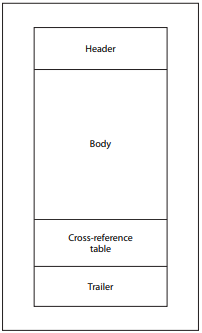
\includegraphics[scale=0.9]{Untitled}
		\centering
		\caption{Struktura objektů}
		\label{fig:pdf}
	\end{figure}

 \section{LaTeX} 
	Vychází z typografického sázecího systému \TeX, který popisuje Pavel Satrapa ve své knize \cite{latex}: \enquote{\textit{Patří do rodiny tak zvaných značkovacích jazyků (markup languages) a dal by se zjednodušeně charakterizovat jako programovací jazyk pro sazbu textů. Jeho základním vstupem je textový soubor, který obsahuje jak sázený dokument, tak příkazy ovlivňující sazbu. Určité znaky mají přiřazen speciální význam a jejich prostřednictvím jsou v textu odlišeny řídicí konstrukce. Typickým příkladem je zpětné lomítko, jímž začínají příkazy.}}
	
	\LaTeX\ je rozšíření \TeX u o balíček přednastavených řídicích konstrukcí. Hlavní cílem těchto systémů je jednoduchost při psaní matematických a jiných vzorců. Ovšem je také velmi oblíben kvůli možnosti jednoduše upravovat dokumenty podle potřeby, přestože prvotní seznámení je ve srovnání s jínymi nástroji ke psaní náročnější.
	
	Základní soubory mají příponu tex kromě souboru s nastavením, ten je ve formátu cls, neboli class file. Tyto soubory mohou být uspořádány do stromové struktury, kde v kořenu stromu je jeden hlavní soubor, do kterého jsou vnořovány další. To napomáhá přehlednosti velkých dokumentů a také používání již vytvořených. 
	
	Soubor se skládá z preambule, která obsahuje nastavení pro celý dokument a případně používané balíčky. Ve druhé části dokumentu se mimo jiné nacházejí kapitoly, sekce a podobně. Základní syntaxe může vypadat takto.
	\newpage
	\begin{verbatim}
	\documentclass{thesis}
	\usepackage{csquotes}
	
	\begin{document}
	Hello world!
	\end{document}
	\end{verbatim}
	
	Výše zmíněné balíčky slouží k přidávání dalších předvytvořených řídících konstrukcí. Tyto balíčky jsou buď nainstalovány zároveň s instalací kompilátoru, nebo je možné je ručně doinstalovávat podle potřeby. 
	
	Pro získání výsledného dokumentu, například ve formátu PDF, je potřeba vše zkompilovat. To provádí kompilátor.  

\section{Moodle a CourseWare}
	Ačkoliv tyto portály se v mnoha aspektech liší, v rámci této práce je můžeme považovat za ekvivalentní. Oba slouží pro podporu studia, a to hlavně v podobě poskytování informací o předmětech studentům, kteří je mají zapsané. Vyučující takto může předat informace o harmonogramu kurzu, přednášky a jiné materiály. Moodle je komplexnější open-source systém s možností upravovat ho k potřebě vzdělávacího zařízení, který navíc poskytuje prostředí pro vytváření a psaní testů, zapisování docházky, komunikaci se studenty a jiné.

\section{FURPS+}
	Vychází z klasifikace požadavků FURPS(\textbf{F}unctionality, \textbf{U}sability, \textbf{R}eliability, \textbf{P}erformance, \textbf{S}upportability) se kterou přišel Robert Grady v roce 1992. Roku 1999 Jacobson at el rozšířili specifikaci o znaménko \enquote{+}, které přidává požadavky a omezení na návrh, implementaci, rozhraní a hardware\cite{furps}. 
	
	\begin{itemize}
		\item Funkční požadavky
			\begin{itemize}
				\item Fukčnost(Functionality) - Požadavky popisující všechny hlavní prvky produktu i důležité aspekty z pohledu architektury např. lokalizovaný systém pro více jazyků.
			\end{itemize}
		\item Nefunkční požadavky
			\begin{itemize}
				\item Použitelnost (Usability) - Zaměřuje se na uživatelskou přívětivost nejenom samotné aplikace, ale i dokumentace týkající se estetiky a konzistence.
				\item Spolehlivost (Reliability) - Spolehlivost systému v podobě doby běhu, správnosti fungování a četnosti výpadků.
				\item Výkon (Performance) - Vypovídá o výkonnosti systému, jak rychle dokáže zpracovávat požadavky, spustit se atd.
				\item Podporovatelnost (Supportability) - Popisuje testovatelnost, škálovatelnost, konfigurovatelnost...
				\item Návrh (Design) - Omezení na návrh systému např. požadavek na relační databázi
				\item Implementace (Implementation) - Specifikuje typ programovacího jazyku, platformu apod.
				\item Rozhraní (Interface) - Komunikace s externími systémy
				\item Fyzické (Physical) - Definuje požadavky na hardware, na kterém daný software poběží, i co se týče fyzické velikosti
			\end{itemize}
	\end{itemize}
	
	Toto rozdělení nám pomáhá identifikovat požadavky. Přispívá k vyšší kvalitě systému a snižuje pravděpodobnost přehlédnutí funkcionality. Právě díky těmto vlastnostem je velmi oblíbené a využívané k vývoji jakéhokoliv software. 